\documentclass[11pt, numbers=endperiod, parskip=half]{scrartcl}

\usepackage{amsmath}
\usepackage{graphicx}
\usepackage[final]{pdfpages}
\usepackage{pdflscape}
\usepackage{minted}
\usepackage{geometry}

\title{Assignment 7}
\subtitle{COS30023 - Languages in Software Development}
\author{Daniel Parker - 971328X}

\date{\today}

\begin{document}
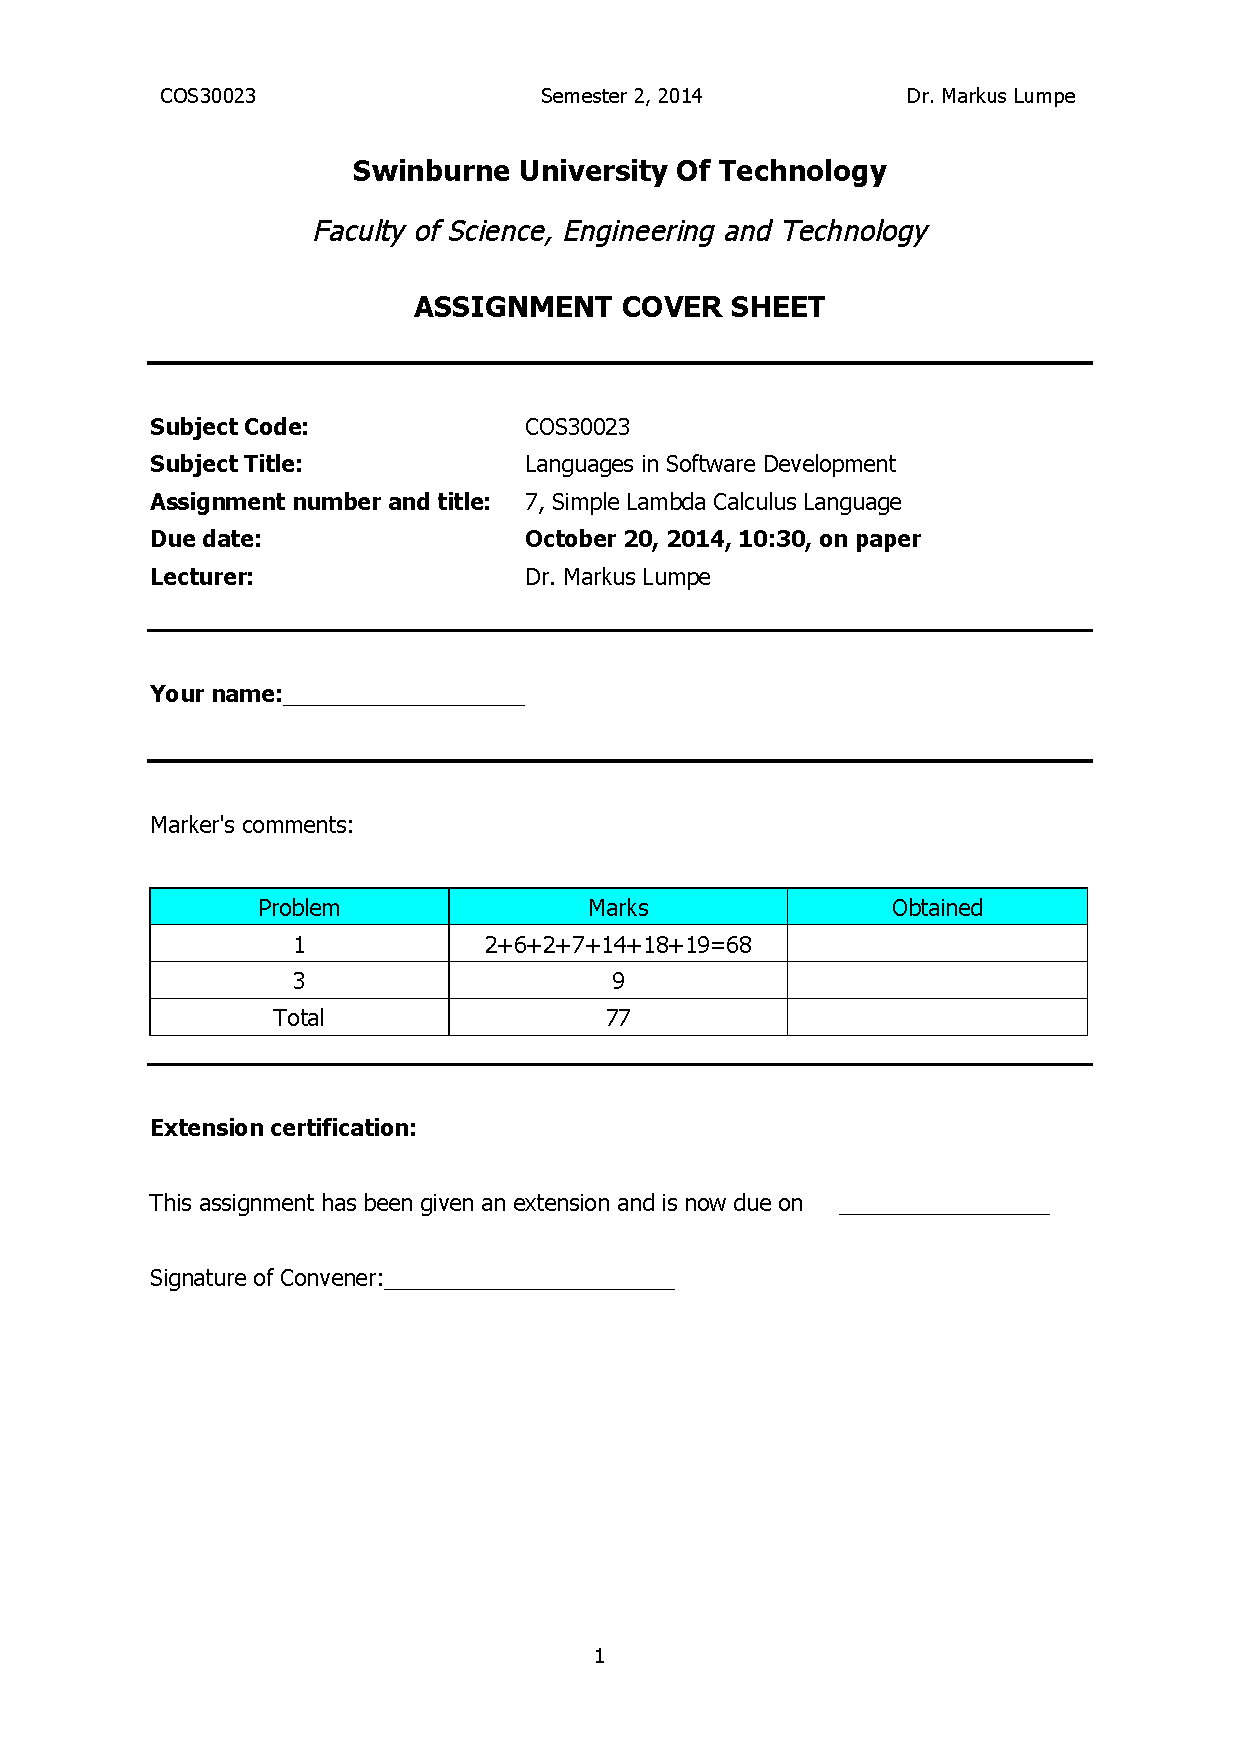
\includepdf[pages=1-1]{ProblemSet7.pdf}
\newgeometry{left=2.5cm}
\maketitle
% \begin{landscape}
\section{LCLParser (Problems 1 \& 2)}
\subsection{LCLParser.jj}
\inputminted[tabsize=2]{java}{LCLParser/src/LCLParser.jj}

\subsection{ast.LCLExpression}
\inputminted[tabsize=2]{java}{LCLParser/src/ast/LCLExpression.java}

\subsection{ast.LCLDeclaration}
\inputminted[tabsize=2]{java}{LCLParser/src/ast/LCLDeclaration.java}

\subsection{ast.LambdaFunction}
\inputminted[tabsize=2]{java}{LCLParser/src/ast/LambdaFunction.java}

\subsection{ast.LambdaNumber}
\inputminted[tabsize=2]{java}{LCLParser/src/ast/LambdaNumber.java}

\subsection{ast.LambdaVariable}
\inputminted[tabsize=2]{java}{LCLParser/src/ast/LambdaVariable.java}

\subsection{ast.LoadDeclaration}
\inputminted[tabsize=2]{java}{LCLParser/src/ast/LoadDeclaration.java}

\subsection{ast.LambdaApplication}
\inputminted[tabsize=2]{java}{LCLParser/src/ast/LambdaApplication.java}

\subsection{ast.IfThenElse}
\inputminted[tabsize=2]{java}{LCLParser/src/ast/IfThenElse.java}

\subsection{ast.Increment}
\inputminted[tabsize=2]{java}{LCLParser/src/ast/Increment.java}

\subsection{ast.Decrement}
\inputminted[tabsize=2]{java}{LCLParser/src/ast/Decrement.java}

\subsection{ast.Zero}
\inputminted[tabsize=2]{java}{LCLParser/src/ast/Zero.java}

\subsection{ast.NotZero}
\inputminted[tabsize=2]{java}{LCLParser/src/ast/NotZero.java}

\restoregeometry
\section{Result}
\begin{minted}{text}
((plus 1) 1) = 2
\end{minted}

\end{document}
